\documentclass[a4paper,11pt,twoside,openright]{report}
\usepackage{standalone}
\usepackage[lmargin=142pt,rmargin=95pt,tmargin=127pt,bmargin=123pt]{geometry}
\usepackage[titleformat=italic,commabeforerest,citefull=first,oxford,super,dotafter=bibentry,see,bibformat=ibidem,human]{jurabib}
\usepackage{csvsimple}
\usepackage{graphicx}
\usepackage{caption}
\usepackage{subcaption}
\usepackage[table]{xcolor}
\usepackage[online,flushleft]{threeparttable}
\usepackage{multirow}
\usepackage{makecell}
\usepackage[super]{nth}
\usepackage[most]{tcolorbox}
\usepackage{listings}
\usepackage{float}
\usepackage{enumitem}
\usepackage{fdsymbol}
\usepackage{awesomebox}
\usepackage{titlesec}
\usepackage[hidelinks]{hyperref}
%\usepackage{inconsolata}
\usepackage{tikz}
\usepackage{tkz-euclide}
\usetikzlibrary{intersections,shapes.arrows,arrows.meta}
\lstset{aboveskip=18pt,belowskip=18pt}
\tcbset{colframe=blue!50!black,colback=blue!20}
\hypersetup{
%   colorlinks=false,
%    linkcolor=blue,
%    filecolor=magenta,
%    urlcolor=cyan,
    pdftitle={PAL-1 Sprite Colour Graphics Adapter},
    pdfpagemode=UseThumbs,
    pdfauthor={Plastic Objects Limited}
}
\renewcommand{\arraystretch}{1.1}
\renewcommand*{\biburlprefix}{\jblangle{}}
\renewcommand*{\bibbudcsep}{~}
\renewcommand\bibname{References}
\AddTo\bibsenglish{\renewcommand*{\urldatecomment}{accessed }}
\titleformat{\chapter}{\normalfont\huge}{\thechapter.}{20pt}{\huge\it}
\makeatletter
\newcommand{\code}{\texttt}
\newcommand\frontmatter{
  \cleardoublepage
  \pagenumbering{roman}}
\newcommand\mainmatter{
  \cleardoublepage
  \pagenumbering{arabic}}
\newcommand\encircle[1]{
  \tikz[baseline=(X.base)]
  \node (X) [draw, shape=circle, inner sep=0] {\strut #1};}
\title{PAL-1 Sprite Colour Graphics Adapter}
\author{Plastic Objects Limited}
\date{}
\begin{document}
\frontmatter
\begin{titlepage}
\begin{figure}[t]
\centering
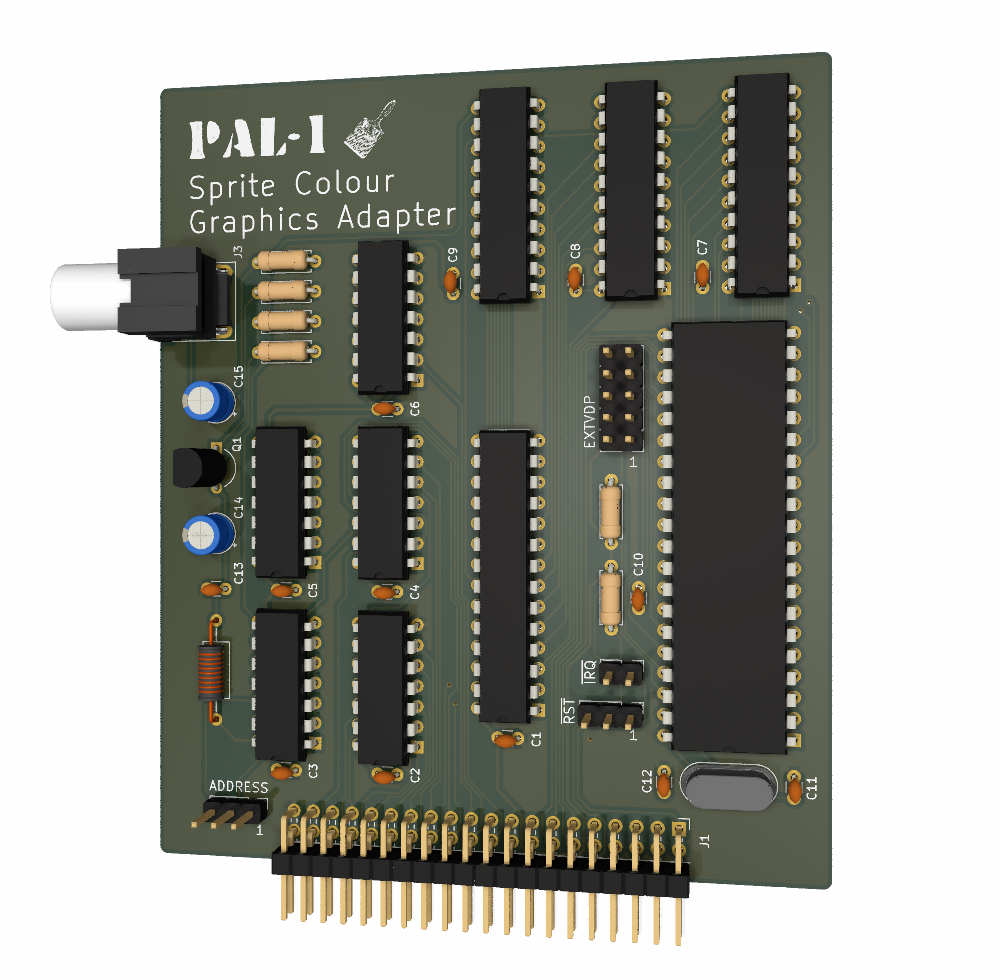
\includegraphics[scale=0.4]{images/video.png}
\end{figure}
\maketitle
\end{titlepage}
\clearpage
\noindent Published by \textbf{Plastic Objects Limited} \\
Beccles, UK

\bigskip
\noindent September 2024
\vfill
{\noindent\Large\textbf{Disclaimer}}
\vskip 6pt
Every effort has been made to ensure the accuracy of the information contained in this document. The information presented within is accurate at the time of publication. Whilst every effort is made to provide accurate information, no warranty or fitness is provided or implied, and the authors and publishers shall have neither liability nor responsibility to any person or entity with respect to any loss or damages arising from its use.

All trademarks, logos and brand names are the property of their respective owners. All company, product and service names mentioned in this document are for identification purposes only. Use of these names, trademarks and brands does not imply endorsement.

\thanks{PAL-1 and the PAL-1 logo used with kind permission by Liu Ganning.}
\clearpage
\tableofcontents
\listoffigures
\cleardoublepage
\chapter*{Introduction}
\addcontentsline{toc}{chapter}{Introduction}
The PAL-1 Sprite Colour Graphics Adapter (SCGA) is an expansion module for the PAL\nobreakdash-1 system\cite{ganning1} based on the Texas Instruments TMS9918A Video Display Processor (VDP)\cite{texas1}. The TMS9918A VDP was used in video systems to provide data display on raster scanned colour television sets or monitors. The IC generates all necessary video, control, and synchronisation signals and also controls the storage and retrieval of display data in its own dedicated screen memory.

\awesomebox[blue]{2pt}{\faInfoCircle}{blue}{The TMS9918A VDP generates a 525-line NTSC encoded colour video signal. While the TMS9928A VDP, which is intended for use with PAL video systems, is functionally compatible with the TMS9918A, it is not pin-for-pin compatible. Thus it is not possible to use the TMS9928A VDP in the PAL-1 Sprite Colour Graphics Adapter. Instead, users who do not have access to an NTSC TV or monitor are recommended to use AV to HDMI or AV to VGA converters as appropriate. Such converters are widely available from the usual e-commerce and auction web sites.}

This expansion module was inspired by a Ciarcia's Circuit Cellar project for a `High-Resolution Sprite-Oriented Color Graphics' expansion card for the Apple II computer, published in BYTE magazine.\cite[pp. 57--80]{byte1} The design for the PAL-1 SCGA also incorporates Static RAM (SRAM) circuitry based on work by Tom LeMense and Dan Werner.\cite{lemense1}\textsuperscript{,}\cite{werner1}

\section*{Overview of the TMS9918A VDP}
The TMS9918A VDP contains all necessary circuitry to generate a video display with up to 16 colours and a maximum resolution of 256 x 192 pixels. Additionally, the VDP supports the display of up to 32 sprites. The image displayed on the screen can best be envisioned as a number of display planes sandwiched together, where each plane has a different priority. For an entity on a specific plane to show through, all planes with higher priorities must be transparent at that point (see Figure \ref{fig:planes}).

\begin{figure}[h!]
	\centering
    \begin{subfigure}[b]{0.4\textwidth}
		\centering
			\scalebox{0.1}{
			\begin{tikzpicture}[font=\sffamily]
				\foreach \p [
				count=\q,
				evaluate=\q as \r using 9-\q
				] in {0,1,2,31,{Pattern plane (text \& graphics)},{Backdrop (solid colour)},{External VDP input},{Black plane}} {
					\def\c{white}
					\ifnumequal{\q}{1}{\def\c{black}}{}
					\ifnumequal{\q}{3}{\def\c{gray!40}}{}
					\draw [line width=4,fill=\c] (\r*6+2.25,\r*5+5) rectangle ++(16,12);
					\draw (\q*6+18.5, \q*5+6) node[anchor=west,scale=8]{\p};
				}
				\foreach \q in {1,2,3} {
					\draw[fill=black] (\q*1.75+38.5,\q+20.5) circle (.25);
				}
				\draw (34,39) node[anchor=west,scale=6]{Hello world};
				\draw[fill=gray!30,line width=2] (9,11) -- ++(4,0) -- ++(-2,4) -- cycle;
				\begin{scope}[fill=white]
					\fill[clip] (24.25,18) rectangle ++(4,4);
					\draw[line width=2] (25.25,20) circle (2);
				\end{scope}
				\draw[fill=gray!80,line width=2] (31.25,21) rectangle ++(4,4);
				\draw [decorate,decoration={brace,amplitude=26pt,mirror,raise=8ex},line width=4]
				(46,10) -- ++(0,18) node[midway,xshift=30em,scale=8]{Sprite planes};

			\end{tikzpicture}
		}
		\caption{Individual display planes.}
	\end{subfigure}\hfill
    \begin{subfigure}[b]{0.4\textwidth}
		\centering
		\scalebox{0.1}{
			\begin{tikzpicture}[font=\sffamily]
				\draw[line width=4] (-12,60) -- ++(-8,-12) -- ++(-4,8);
				\draw[fill=black!80] (-20,43) circle (6);
				\draw[line width=4,fill=white,rounded corners=0.2cm] (-32,28) rectangle ++(28,20) {};
				\draw[line width=8,rounded corners=1cm,fill=gray!40] (-30,30) rectangle ++(20, 16) {};
				\draw[fill=black] (-12.1,59.9) circle (.3);
				\draw[fill=black] (-24,56) circle (.3);
				\draw[fill=black!60,line width=4] (-7,41) circle (1);
				\draw[fill=black!60,line width=4] (-7,44) circle (1);
				\begin{scope}
					\draw[clip] (-7,41) circle (1);
					\draw[line width=8] (-7.5,40) -- (-6.5,42);
				\end{scope}
				\begin{scope}
					\draw[clip] (-7,44) circle (1);
					\draw[line width=8] (-6.8,43) -- (-7.2,45);
				\end{scope}
				\draw[fill=black!60,line width=2] (-9,31) rectangle ++(4,6);
				\foreach \q in {1, ..., 5}{
					\draw[line width=8, color=black!40] (-8.5,\q+31) -- ++(3,0);
				}
				\draw [color=white,fill=white] (-28,32) rectangle ++(16,12);
				\draw (-26,41) node[anchor=west,scale=6]{Hello world};
				\draw[fill=gray!30,line width=2] (-27,33) -- ++(4,0) -- ++(-2,4) -- cycle;
				\draw[fill=gray!80,line width=2] (-17,33) rectangle ++(4,4);
				\draw[fill=white,line width=2] (-17,37) circle (2);

				\draw[line width=2] (-17,30.5) -- ++(3,-5) -- ++(-1,0) -- ++(3,-5)
				node[scale=8,yshift=-.6em]{Backdrop};
			\end{tikzpicture}
		}
		\caption{Image shown on screen.}
	\end{subfigure}
    \caption[TMS9918A VDP display planes]{TMS9918A VDP overlapping display planes.}
	\label{fig:planes}
\end{figure}

In descending priority order, the display planes are made up of 32 \textit{Sprite Planes}, each of which may contain a single sprite. Below these sprite planes is the \textit{Pattern Plane}, which is used for the display of textual and graphics images. Below this is the \textit{Backdrop Plane}, which provides a single colour border around all other planes and sets the default colour for the active display area. Finally, with the lowest priority is the \textit{External Video Plane}, which displays a video image from a compatible external source (see also appendix \ref{sec:ttlpins}).

The VDP supports four video colour display modes that determine the appearance of the Pattern Plane. In both graphics modes, \textit{Graphics 1} and \textit{Graphics 2}, the pattern plane is split into groups of 8x8 pixels, referred to as pattern positions. Graphics and images using multiple colours may be created by defining unique patterns for each pattern position. In \textit{Text} mode, the Pattern Plane is split into groups of 6x8 pixels, resulting in 40x24 text positions on the screen. Sprites are not displayed in \textit{Text} mode and only two colours are allowed. Finally, in \textit{Multicolor} mode, the screen is split into a grid of 64x48 positions, each of which is 4x4 pixels. In this mode, each position may have a unique colour.

The \textit{Sprite Planes} are used for the display of up to 32 sprites in the \textit{Multicolor} and \textit{Graphics} modes. Sprites are automatically transparent in \textit{Text} mode and thus cannot be used in this mode. Each sprite covers a 8x8, 16x16 or 32x32 pixel area and may be positioned anywhere on its plane. Any part of the plane not covered by the sprite is transparent, as may be all or part of a sprite.

The VDP registers define the base addresses for several sub-blocks within Video RAM (VRAM). The sub-blocks form \textit{tables} which are used to define sprites and produce the desired text or images on the screen. Before use, the contents of these tables must be initialised by applications running on the PAL-1. Displaying text, drawing images and moving sprites across the screen can be achieved by choosing the relevant register parameters and changing the pointers.

\mainmatter
\chapter{Getting Started}
\section*{Board assembly}
Before assembling your PAL-1 Sprite Colour Graphics Adapter board check the package contents against the Bill of Materials on page \pageref{sec:bom}, and contact your distributor as soon as possible if any items are missing.

No specialist tools are required for assembling the board, though care must be taken when handling ESD sensitive components, especially the ICs. Before inserting the ICs into their sockets, check the board for dry joints and solder bridges. Also be sure to pay special attention to the orientation of the ICs, ensuring pin 1 of each IC is correctly aligned. Refer to the board layout on page \pageref{fig:layout} for the orientation of ICs, diodes and electrolytic capacitors.

\section*{Installation and configuration}
\label{sec:configuration}

Because of its width, the PAL-1 Sprite Colour Graphics Adapter cannot be installed in all slots of the PAL-1 Motherboard.\cite{ganning2} Rather, it must be installed in any of slots 4, 5, or 6. Alternatively, it may be directly connected to the PAL-1 using a 40-pin IDC cable.

\awesomebox[red]{2pt}{\faHandPaper}{red}{To prevent damage to your system, \textit{always} power off your PAL-1 before installing or removing the PAL-1 Sprite Colour Graphics Adapter board. Ensure that the pins are correctly aligned when inserting the board into the PAL-1 motherboard or when directly connecting it to the PAL-1 expansion port using an IDC cable.}

\subsection*{Data and register addresses}
The TMS9918A VDP has an 8-bit data bus, which is memory mapped on the PAL-1 system at addresses determined by the position of the \textsf{ADDRESS} jumper, as shown in Table \ref{tab:address}. Up to two PAL-1 Sprite Colour Graphics Adapters can be installed in one system by assigning each adapter unique data and register addresses.

\begin{table}
	\centering
	\sf
	\renewcommand{\arraystretch}{1.1}
	\begin{tabular}{@{\extracolsep{4pt}}ccc@{}}
		\hline
		\textbf{Pins} & \textbf{VDP data} & \textbf{VDP register} \\
		\hline
		\textbf{1 -- 2} & \$16EC & \$16ED \\
		\textbf{2 -- 3} & \$16EE & \$16EF \\
		\hline
	\end{tabular}
	\caption{\textsf{ADDRESS} jumper settings.}
	\label{tab:address}
\end{table}
\subsection*{Option jumpers}
The PAL-1 Sprite Colour Graphics Adapter has two option jumpers to configure its behaviour:

\begin{itemize}
	\item[$\overline{\mbox{RST}}$]
	\begin{description}
		\item[1 -- 2] Disables TMS9918A $\overline{\mbox{RESET}}$/SYNC using pull-up resistor $R1$.
		\item[2 -- 3] Connects the TMS9918A  $\overline{\mbox{RESET}}$/SYNC line with the $\overline{\mbox{RESET}}$ line of the PAL-1 MOS6502 CPU, ensuring it is used as a reset signal on the VDP.
		\item[No jumper] This jumper \textit{must} be removed when using the \textsf{EXTVDP} external video pin header.
	\end{description}
	\item[$\overline{\mbox{INT}}$] Enable CPU interrupts. If enabled, interrupts are raised each time a frame is completed, while the beam is tracing up to the upper left corner of the screen. This occurs every $1/60$\textsuperscript{th} of a second (approximately).
\end{itemize}

\chapter{Sample Code}

Programming the PAL-1 Sprite Colour Graphics Adapter simply requires the ability to write to and read from the memory mapped data and register addresses. Many programming languages provide statements to achieve this, including the \code{POKE} and \code{PEEK} statements in BASIC, and \code{C!} and \code{C@} in Forth.

Note that the examples included below use the default SCGA data and register addresses (\$16EC, $5868_{10}$ and \$16ED, $5869_{10}$).  Further examples may be found on Github at \url{https://github.com/dimitrit/pal1vdp}.

\subsection*{BASIC}

\textsf{TODO!}

%\lstinputlisting[basicstyle=\footnotesize\ttfamily,caption={BASIC example},captionpos=b,
%	language={[Visual]Basic},label={lst:sample1},frame=single]{../src/KNIGHT.BAS}

\subsection*{6502 assembly language}

The assembly language example is taken from the `\textit{High-Resolution Sprite-Oriented Color Graphics}' article in the August 1982 issue of BYTE magazine.\cite[pp. 57--80]{byte1} The code has been modified where required to allow it to run on the PAL-1.

\begin{figure}[h!]
\centering
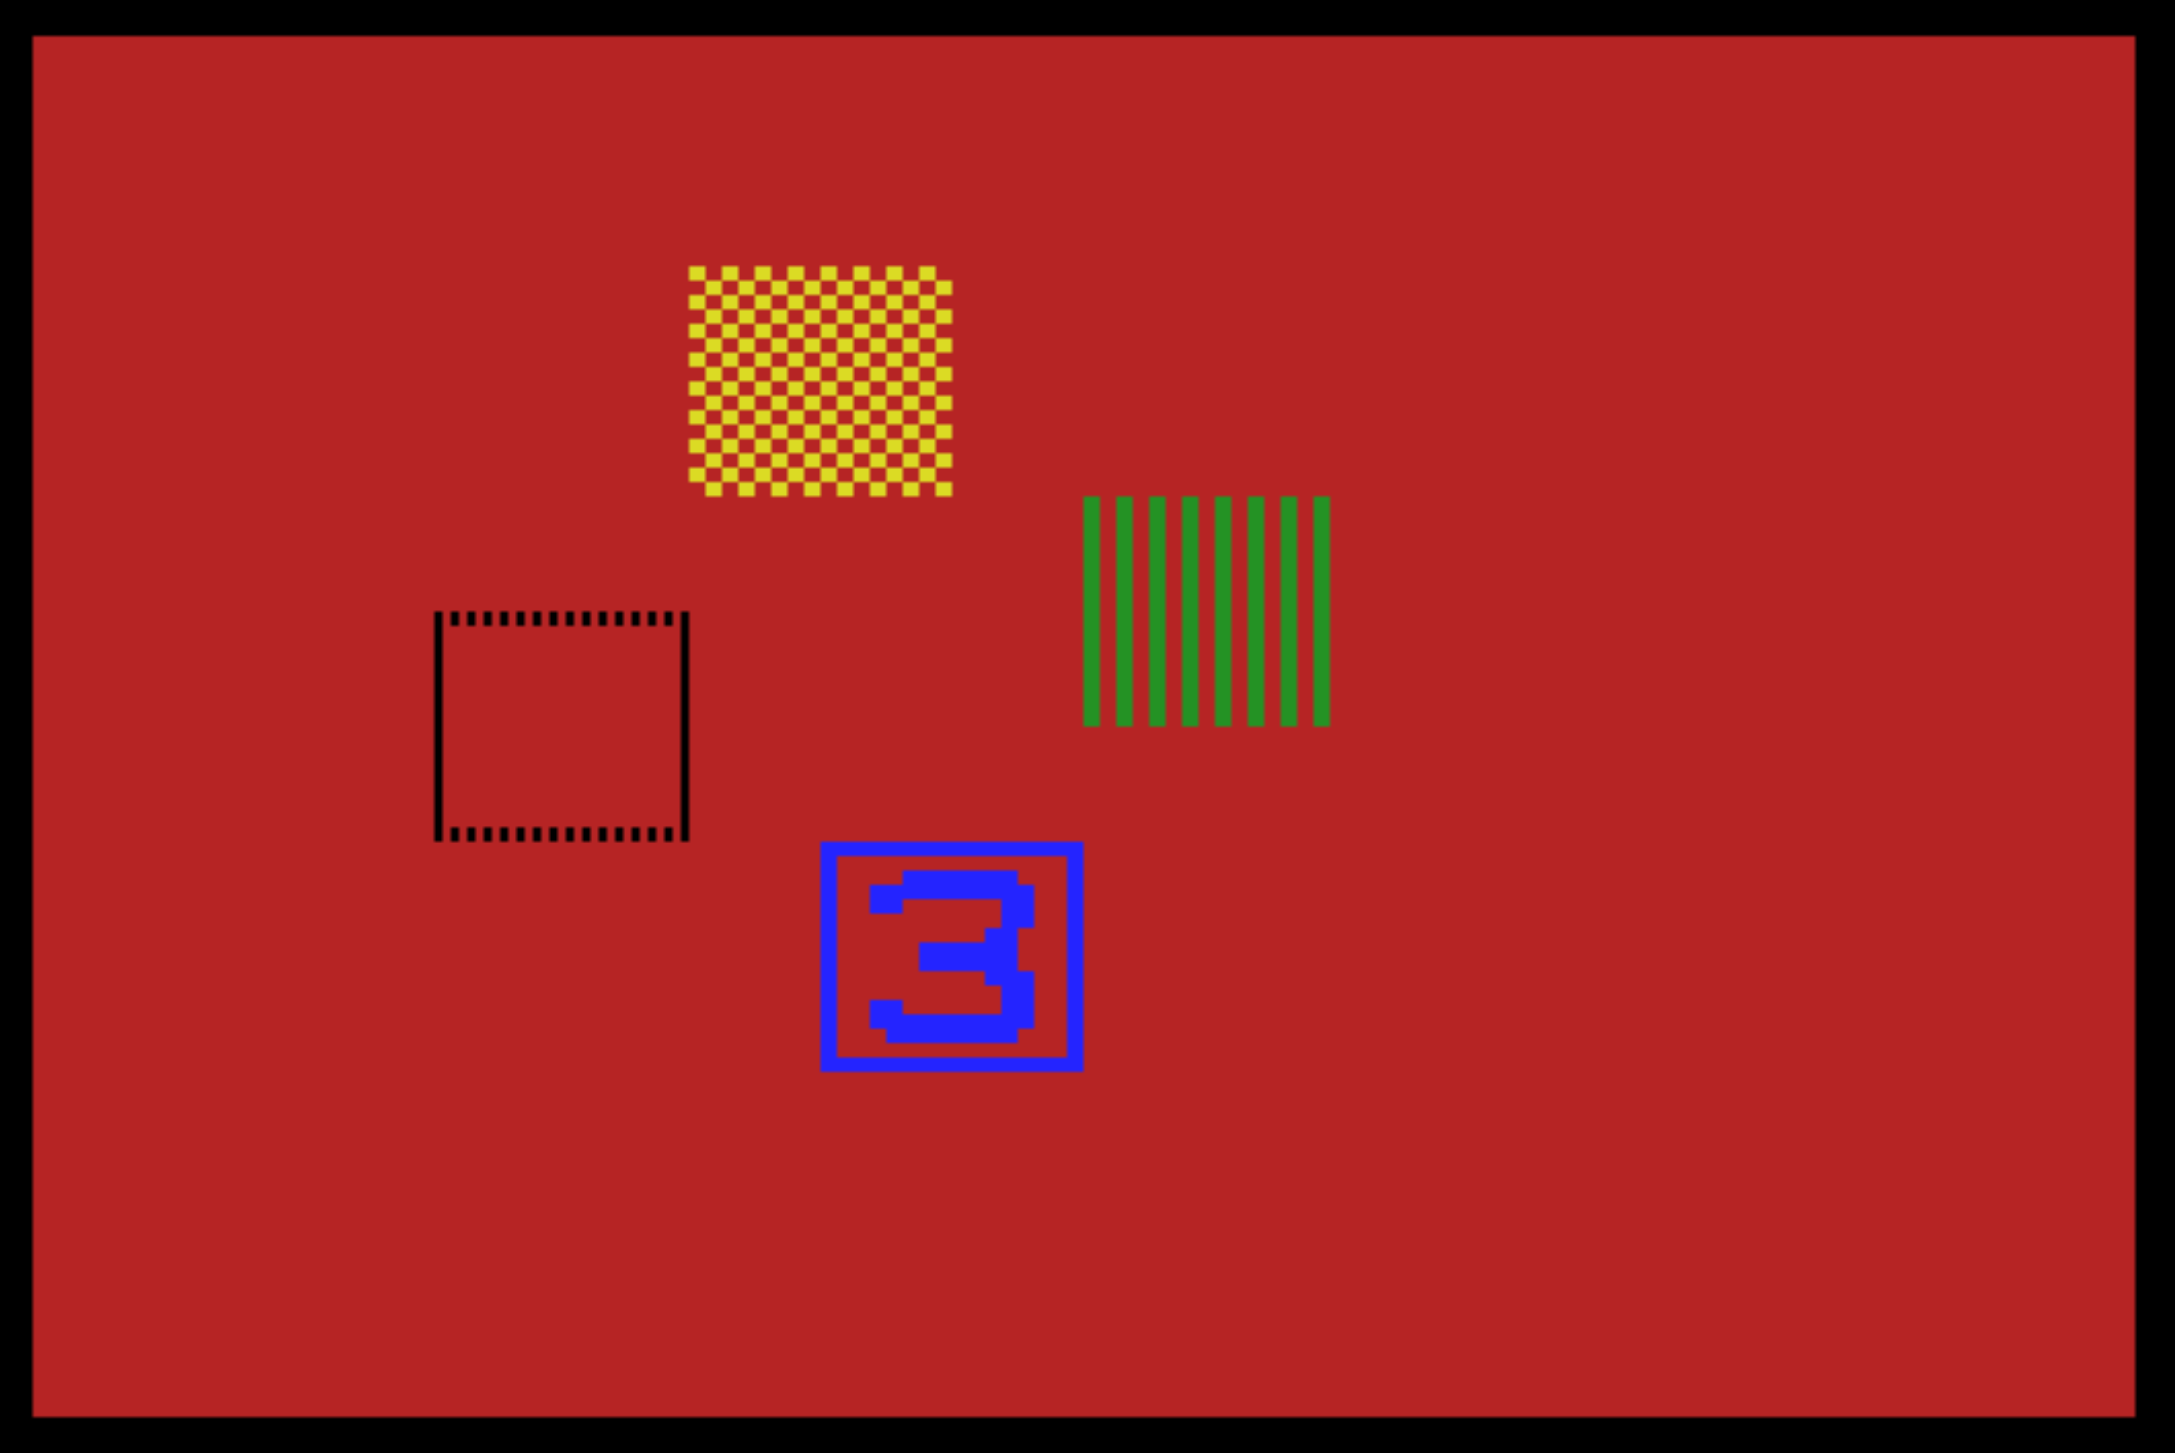
\includegraphics[scale=.7]{images/video-demo.png}
\caption[Assembly language Video Demo showing sprites]{6502 Assembly language \textit{Video Demo} showing four sprites.}
\label{fig:asmdemo}
\end{figure}

The program starts by initialising the eight VDP registers and clearing the VRAM. In this example the 9918A is set to the following operating specifications: Graphics II mode, external video input disabled, and 16 x 16 pixel sprites, with selectable magnification to twice their normal size (32 x 32 pixels) under keyboard control. When the program starts, four different sprites are displayed, as shown in Figure \ref{fig:asmdemo}. The display can be changed as follows. When you press the \textsf{GO} key, the sprites' position coordinates are incremented and the sprites move. Pressing the \textsf{0} key and then a hexadecimal digit \textsf{1} through \textsf{F} will set one of the fifteen background colours or transparency. Pressing the \textsf{AD} or \textsf{DA} keys will vary the size of the sprites between 16 x 16 and 32 x 32 pixels.

\lstinputlisting[basicstyle=\footnotesize\ttfamily,caption={Ciarcia's Circuit Cellar Video Demo},
	captionpos=b,language={[Motorola68k]Assembler},
	label={lst:sample2},frame=single]{../src/ciarcia.a65}

\appendix

\chapter{Connector Pin Outs}
\label{sec:connectors}

\subsection*{External Video Pin Header (\textsf{EXTVDP})}
\label{sec:ttlpins}
The PAL-1 Sprite Colour Graphics Adapter (SCGA) external video pin header (\textsf{EXTVDP}) can be used to connect a compatible external video source. Alternatively, it allows the SCGA to be used as the source for other systems.\cite[pp. 3.7--3.8]{texas1}

Note that the pins of this header are numbered `odd-even' with pin \textsf{1} clearly marked on the PCB, as shown in figures \ref{fig:pinheader} and \ref{fig:layout}. \textbf{Be sure to check the TTL voltage levels and signals before connecting any external systems as incorrect voltages and/or incompatible signals may result in permanent damage to your PAL-1 Sprite Colour Graphics Adapter.}

\begin{figure}[h!]
	\centering
    \begin{minipage}[b]{\linewidth}
	    \centering
		\scalebox{0.1}{
			\begin{tikzpicture}[font=\sffamily]
				\draw (3,5.5) node[scale=12, rotate=-90,color=gray]{1};
				\draw (5.5,17) node[scale=12,anchor=west,color=gray]{EXTVDP};
				\draw [line width=8] (6,4) -- ++(0,9);
				\draw [line width=8] (6,13)
				\foreach \q in {1, ..., 5} { -- ++(1,1) -- ++(4,0) -- ++(1,-1) } -- ++(0,-9)
				\foreach \q in {5, ..., 1} {	-- ++(-1,-1) -- ++(-4,0) -- ++(-1,1) } -- cycle;
				\foreach \q [
						evaluate=\q as \odd using int(\q*2-1),
						evaluate=\q as \even using int(\q*2)
				] in {5, ..., 1} {
					\draw [fill=black] (\q*6+2.25,5.5) rectangle ++(1.5,1.5);
					\draw [fill=black] (\q*6+2.25,10) rectangle ++(1.5,1.5);

					\draw (3+\q*6, 16.5) node[scale=8]{\even};
					\draw (3+\q*6, 0.5) node[scale=8]{\odd};
				}
			\end{tikzpicture}
		}
		\captionof{figure}[External video pin header]{\textsf{EXTVDP} external video pin header.}
		\label{fig:pinheader}
	\end{minipage}
	~\par\bigskip
    \begin{minipage}[b]{\linewidth}
			\renewcommand{\arraystretch}{1.1}
			\centering
			\begin{tabular}{@{\extracolsep{4pt}}clp{80mm}@{}}
				\hline
				Pin & Signal & Description \\
				\cline{1-3}
				1 & GND & Ground  \\
				2 & VCC & +5V Supply Voltage \\
				3 & GND & Ground  \\
				4 & COMVID & Composite Video Output \\
				5 & GROMCLK & VDP Output Clock $= XTAL/24$ \\
				6 & COMVID & Composite Video Output \\
				7 & EXTVDP & External Video (VDP) Input \\
				8 & CPUCLK &  VDP Colour Burst Frequency Clock \\
				9 &  $\overline{\mbox{RESET}}$/SYNC & This is a tri-level input pin. When it is below 0.8 volts, $\overline{\mbox{RESET}}$/SYNC initialises the VDP. When it is above 9 volts $\overline{\mbox{RESET}}$/SYNC is the synchronising input for external video. \\
				10 & COMVID\textsubscript{r} & Unconditioned Composite Video Output of the TMS9918A VDP. \\
				\hline
			\end{tabular}

		\captionof{table}[External video pin header]{\textsf{EXTVDP} external video pin header.}
		\label{tab:ttlpins}
	\end{minipage}
\end{figure}

\chapter{Schematic}
\label{sec:schematic}

\begin{figure}[h!]
	\centering
	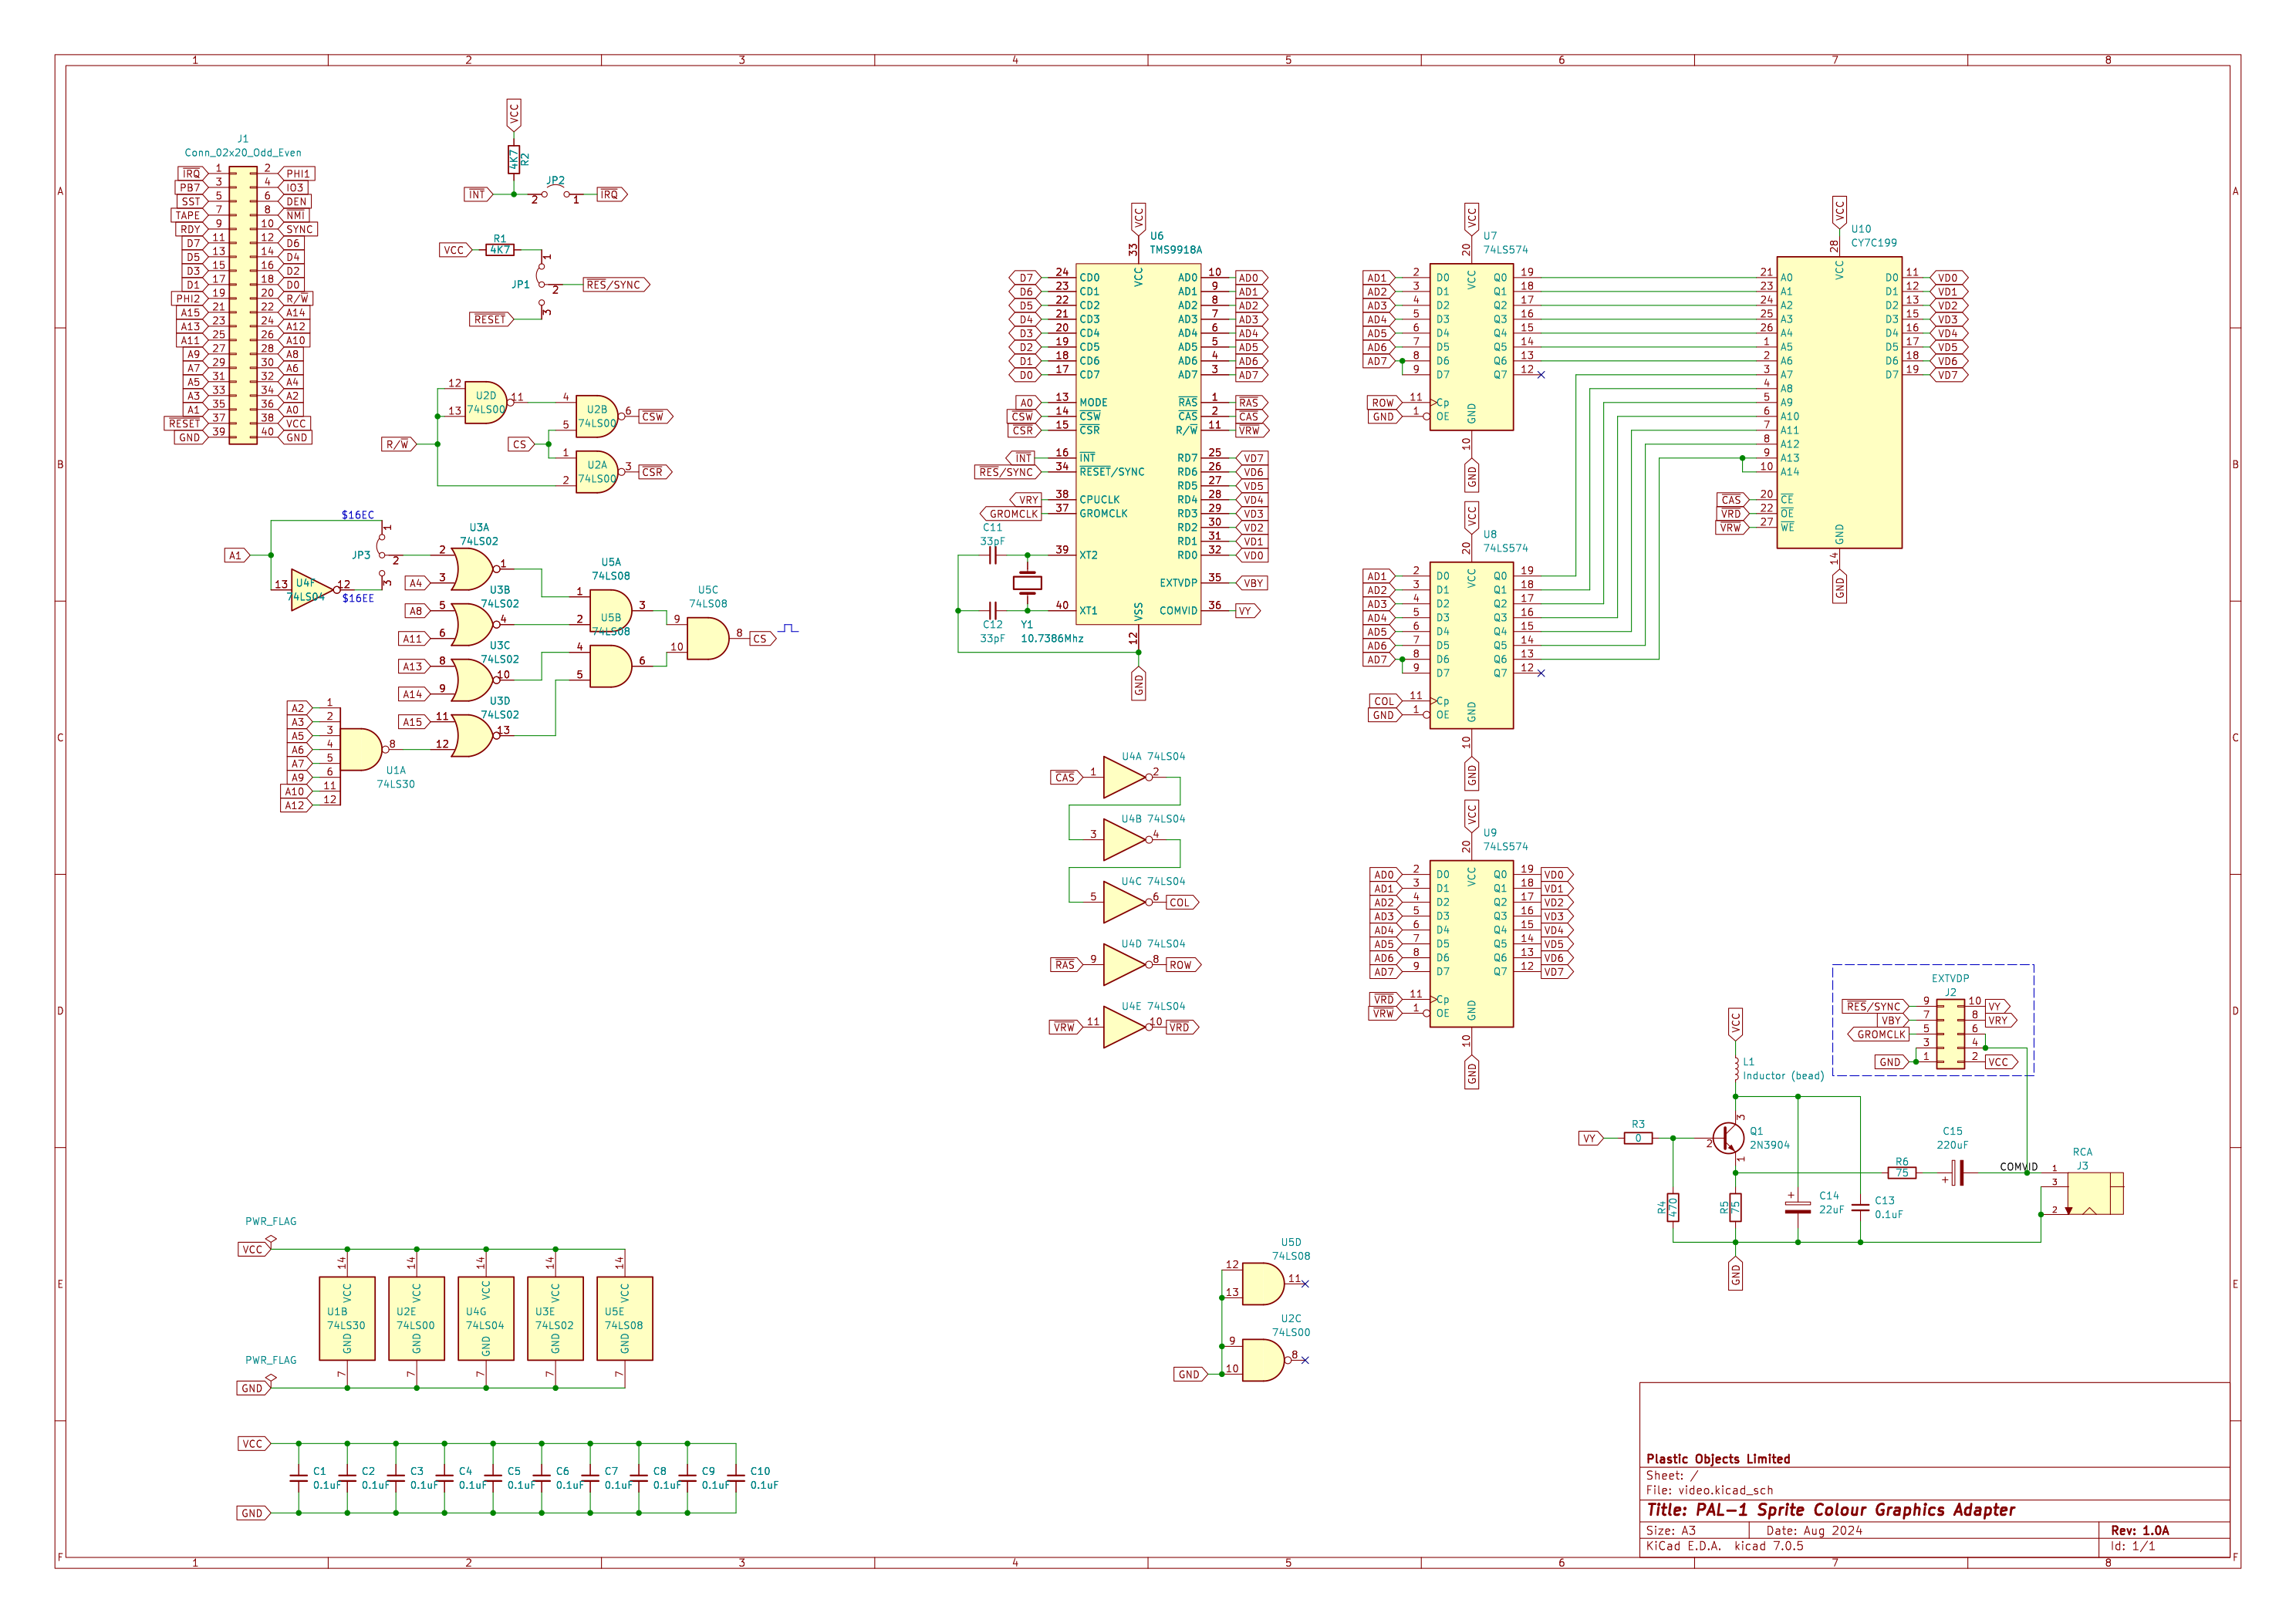
\includegraphics[scale=.24,angle=90,origin=c]{images/scga-schematic-1.0a.png}
	\caption[Sprite Colour Graphics Adapter schematic]{PAL-1 Sprite Colour Graphics Adapter schematic.}
	\label{fig:layout}
\end{figure}

\chapter{Board layout}
\begin{figure}[h!]
\centering
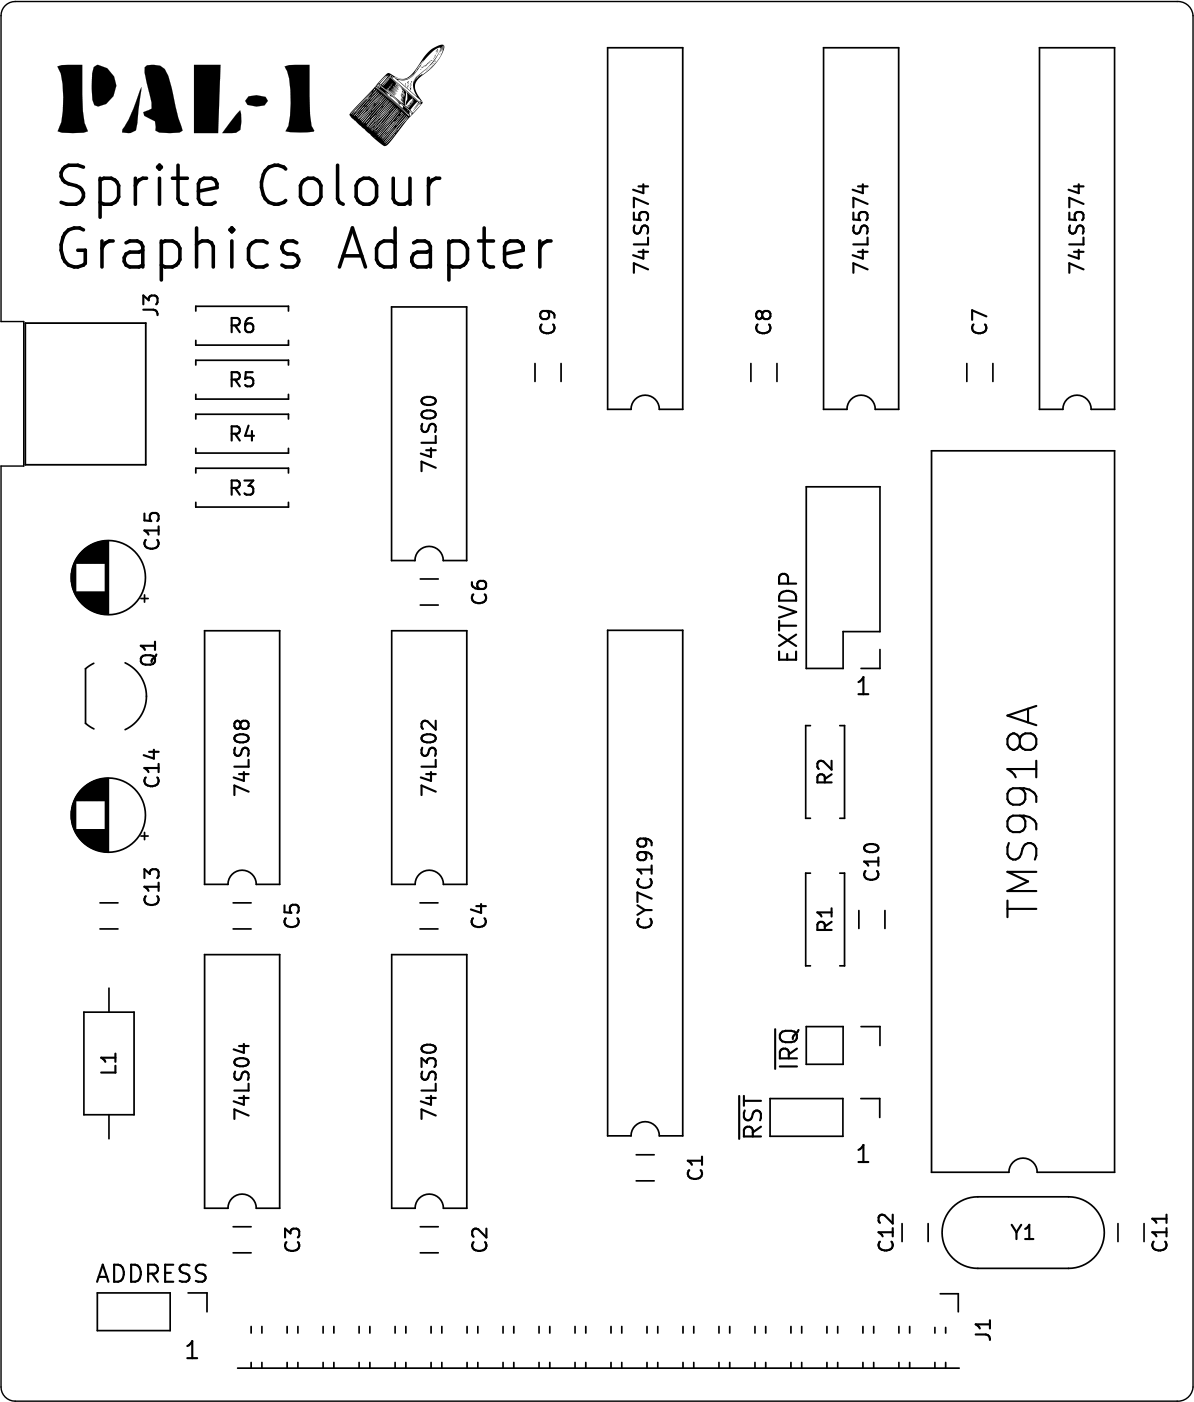
\includegraphics[scale=.25]{images/scga-brd-1.0a.png}
\caption[Sprite Colour Graphics Adapter component locations]{PAL-1 Sprite Colour Graphics Adapter component locations.}
\label{fig:layout}
\end{figure}

\chapter{Bill of Materials}
\label{sec:bom}

\begin{table}[htb]
	\csvreader[head to column names,
	separator=semicolon,
	tabular={| c | c | c | p{7cm} |},
	table head=\hline\rowcolor{gray!20}\textbf{Part} & \textbf{Qty} & \textbf{Value} & \textbf{Description}\\\hline,
	late after last line=\\\hline]{scga-bom-1.0a.csv}{}
	{\Ref&\Qnty&\Value&\Description}
	\caption[Sprite Colour Graphics Adapter bill of materials]{PAL-1 Sprite Colour Graphics Adapter v1.0A bill of materials.}
	\label{tab:bom}
\end{table}

\bibliography{scga}
\bibliographystyle{jox}
\addcontentsline{toc}{chapter}{References}

\end{document}